\documentclass{article}
\usepackage{graphicx}
\usepackage[utf8]{ctex}
\usepackage{amsmath}
\usepackage[fontsize=10pt]{fontsize}
\usepackage{geometry}
\geometry{a4paper,left=0.75in,right=0.75in,top=1in,bottom=0.75in}
\usepackage{setspace}
\setlength{\parindent}{0em}
\def\kong{\hspace*{2em}}
\usepackage{amsfonts,amssymb}
\usepackage{xcolor}
\usepackage{fontspec}
\usepackage{enumitem}
\linespread{1.5}
\usepackage{hyperref}
\usepackage{hyperref}
\hypersetup{hidelinks,
	colorlinks=true,
	allcolors=black,
	pdfstartview=Fit,
	breaklinks=true}

\usepackage{listings}
	\lstset{
 columns=fixed,
 numbers=left,
 numberstyle=\tiny\color{gray},
 frame=none,
 backgroundcolor=\color[RGB]{245,245,244},
 keywordstyle=\color[RGB]{40,40,255},
 numberstyle=\footnotesize\color{darkgray},
 commentstyle=\it\color[RGB]{0,96,96},
 stringstyle=\rmfamily\slshape\color[RGB]{128,0,0},
 showstringspaces=false,
 language=c,
 basicstyle=\ttfamily
	}

\usepackage{fancyhdr}

\pagestyle{fancy}
\fancyhf{}
\fancyhead[LE,RO]{\thepage}
\fancyhead[RE,LO]{\kaishu PB21000276施耀炜}



\date{2022年3月}

\begin{document}

\setcounter{page}{1}
\thispagestyle{empty}
\kong
\\[10pt]
\begin{center}
	\textbf{\huge \heiti 实验报告三}\\[6pt]
    \textbf{\huge \heiti 直流电源特性实验}\\[12pt]
	\textbf{学号：}\underline{\kaishu PB21000276} \qquad 
    \textbf{姓名：}\underline{\kaishu 施耀炜} \qquad 
    \textbf{班级：}\underline{\kaishu 21级少院6班}\qquad 
    \textbf{日期：}\underline{2022年4月13日}\\[24pt]
\end{center}
\section{实验名称}
    \kong 直流电源特性实验
\section{实验目的}
    \kong 掌握直流电源特性的测量方法，了解负载对电源输出特性的影响，
    掌握非线性内阻电源开路电压和短路电流的测量方法。
\section{实验原理}
    \subsection{纹波系数}
    \kong 直流稳压电源不可避免地在直流稳定量中带有一些交流成分，
    这种叠加在直流稳定量上的交流分量就称之为纹波。
    纹波系数是指负载上交流电压的有效值与直流电压之比，是表征直流电源品质的一个重要参数。
    $$
        \text{纹波系数}K_{u}=\frac{U_\text{交流电压有效值}}{U_\text{直流电压}}\times 100\% \eqno{(3.1)}
    $$
    \subsection{电源开路电压和短路电流}
    \kong 开路电压是指电源在断路时的输出电压值，短路电流是指外电源短路时的最大电流。
    对于有些具有非线性内阻的电源，不适用 $U-I$ 曲线外推法进行测量，
    故采用等效电路或补偿法来进行测量，电路图如下：
    \begin{figure}[htp]
        \centering
        \textbf{图\ 3.1}\quad 等效电路法测量开路电压（左）和短路电流（右）电路图\\
        
\includegraphics[width=12cm]{tp1.png}
    \end{figure} 
%实验仪器
\section{实验仪器}
    \begin{itemize}[noitemsep]
        \item 信号发生器
        \item 数字电压表（直流电压档、交流电压档）
        \item 检流计
        \item 电阻箱
        \item 滑线变阻器
        \item 微安表
        \item 电源
        \item 电池
        \item 面包板（整流二极管、电容、电阻）
        \item 导线
    \end{itemize}
%数据处理与分析
\section{实验与数据处理分析}
    \subsection{不同负载下负载功率和纹波系数的测量}
        \kong 信号源选定 $500Hz$，$Vp-p=10V$，正弦交流信号，负载$R_L$接电阻箱，在$20\sim 2000\Omega$范围内测量该电源的负载功率和纹波系数曲线。
        \subsubsection{$\pi$型全波整流滤波电路}
        \kong 电容选用$1\mu F$，在面包板上连接$\pi$型全波整流滤波电路，数据和曲线如下。
        \begin{figure}[htp]
            \centering
            \textbf{表\ 3.1}\quad 电容$1\mu F$ 下 $\pi$型全波整流电路的测量数据  \\[4pt]
            
\includegraphics[width=12cm]{bg1.png}
        \end{figure}
        \newpage
        \begin{minipage}{0.49\linewidth}
            \centering
            \textbf{图\ 3.2}\quad $1\mu F$ 下 $\pi$型全波整流电路$R-P$图  \\[4pt]
            
\includegraphics[width=1\linewidth]{tp2.png}
            \label{tp2.png} 
        \end{minipage}
        %\qquad
        \begin{minipage}{0.49\linewidth}
            \centering
            \textbf{图\ 3.3}\quad $1\mu F$ 下 $\pi$型全波整流电路$R-K$图  \\[4pt]
            
\includegraphics[width=1\linewidth]{tp3.png}
            \label{tp3.png}
        \end{minipage}
        根据测量结果，负载$R=1450\Omega$附近时，功率$P$最大，约为$2.34\rm{W}$。
        \subsubsection{单个$10\mu F$电容型全波整流滤波电路}
        \kong 电容选用$10\mu F$，在面包板上连接单个电容型全波整流滤波电路，数据和曲线如下。
        \begin{figure}[htp]
            \centering
            \textbf{表\ 3.2}\quad 电容$10\mu F$ 下 单个电容型全波整流电路的测量数据  \\[4pt]
            
\includegraphics[width=12cm]{bg2.png}
        \end{figure}
        \newpage 
        \begin{figure}[htp]
            \centering
            \textbf{图\ 3.4}\quad $10\mu F$ 下 单个电容型全波整流电路$R-P$图  \\[4pt]
            
\includegraphics[width=15cm]{tp4.png}
        \end{figure}
        \begin{figure}[htp]
            \centering
            \textbf{图\ 3.5}\quad $10\mu F$ 下 单个电容型全波整流电路$R-K$图  \\[4pt]
            
\includegraphics[width=15cm]{tp5.png}
        \end{figure}
        根据测量结果，负载$R=80\Omega$附近时，功率$P$最大，约为$20.35\rm{W}$。\\[12pt]
        \kong 对比两种不同的全波整流滤波电路，可以看到，在相同负载时，
        $1\mu F$ 下 $\pi$型全波整流电路相比$10\mu F$ 下 单个电容型全波整流电路，直流电压较小，同时纹波系数也更小。
    \subsection{非线性内阻电源开路电压和短路电流的测定}
        \kong 测量待测电源 $E_x$ 的开路电压和短路电流，并计算 $E_x$ 内阻。\\
        \kong 测得开路电压$U=1.5927V$，短路电流$I=5.14mA$，内阻$r=\displaystyle{\frac{U}{I}}=309.86\Omega$，实验情况如下图。\\
        \newpage
        \begin{minipage}{0.49\linewidth}
            \centering
            \textbf{图\ 3.6}\quad 开路电压的测量实验实拍  \\[8pt]
            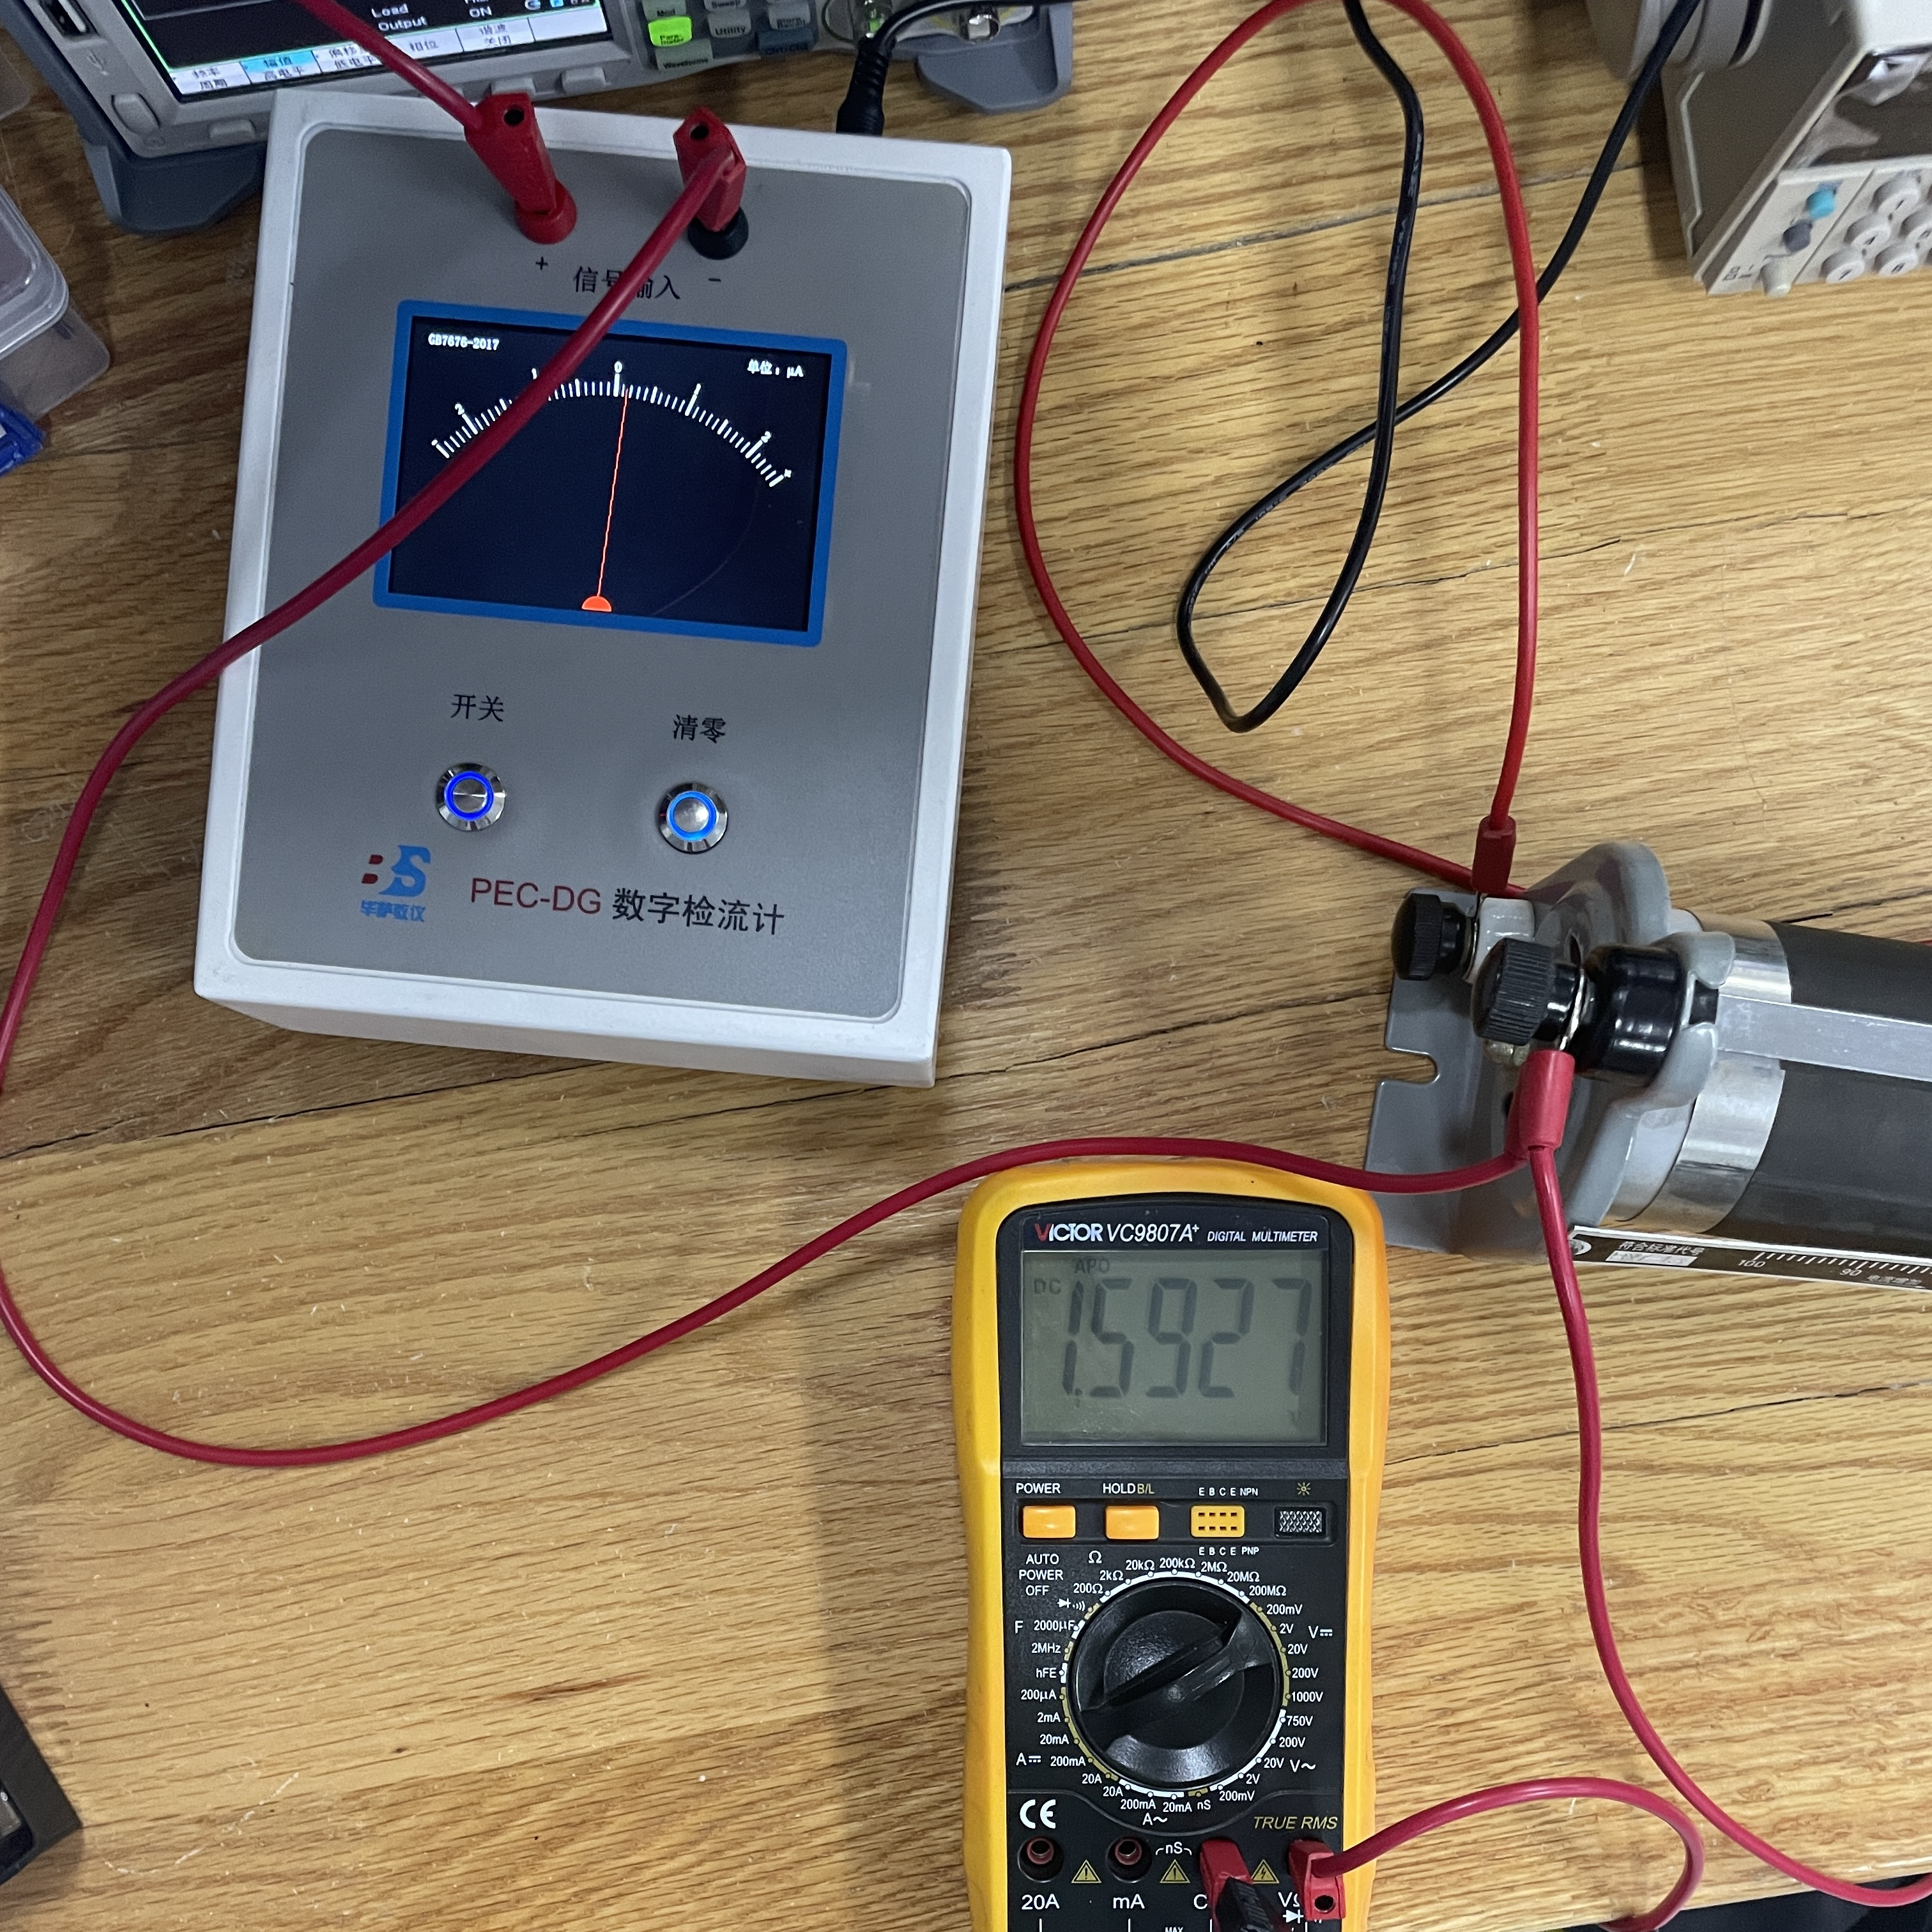
\includegraphics[width=0.95\linewidth]{tp6.jpg}
            \label{tp6.png}  
        \end{minipage}
        %\qquad
        \begin{minipage}{0.49\linewidth}
            \centering
            \textbf{图\ 3.7}\quad 短路电流的测量实验实拍  \\[8pt]
            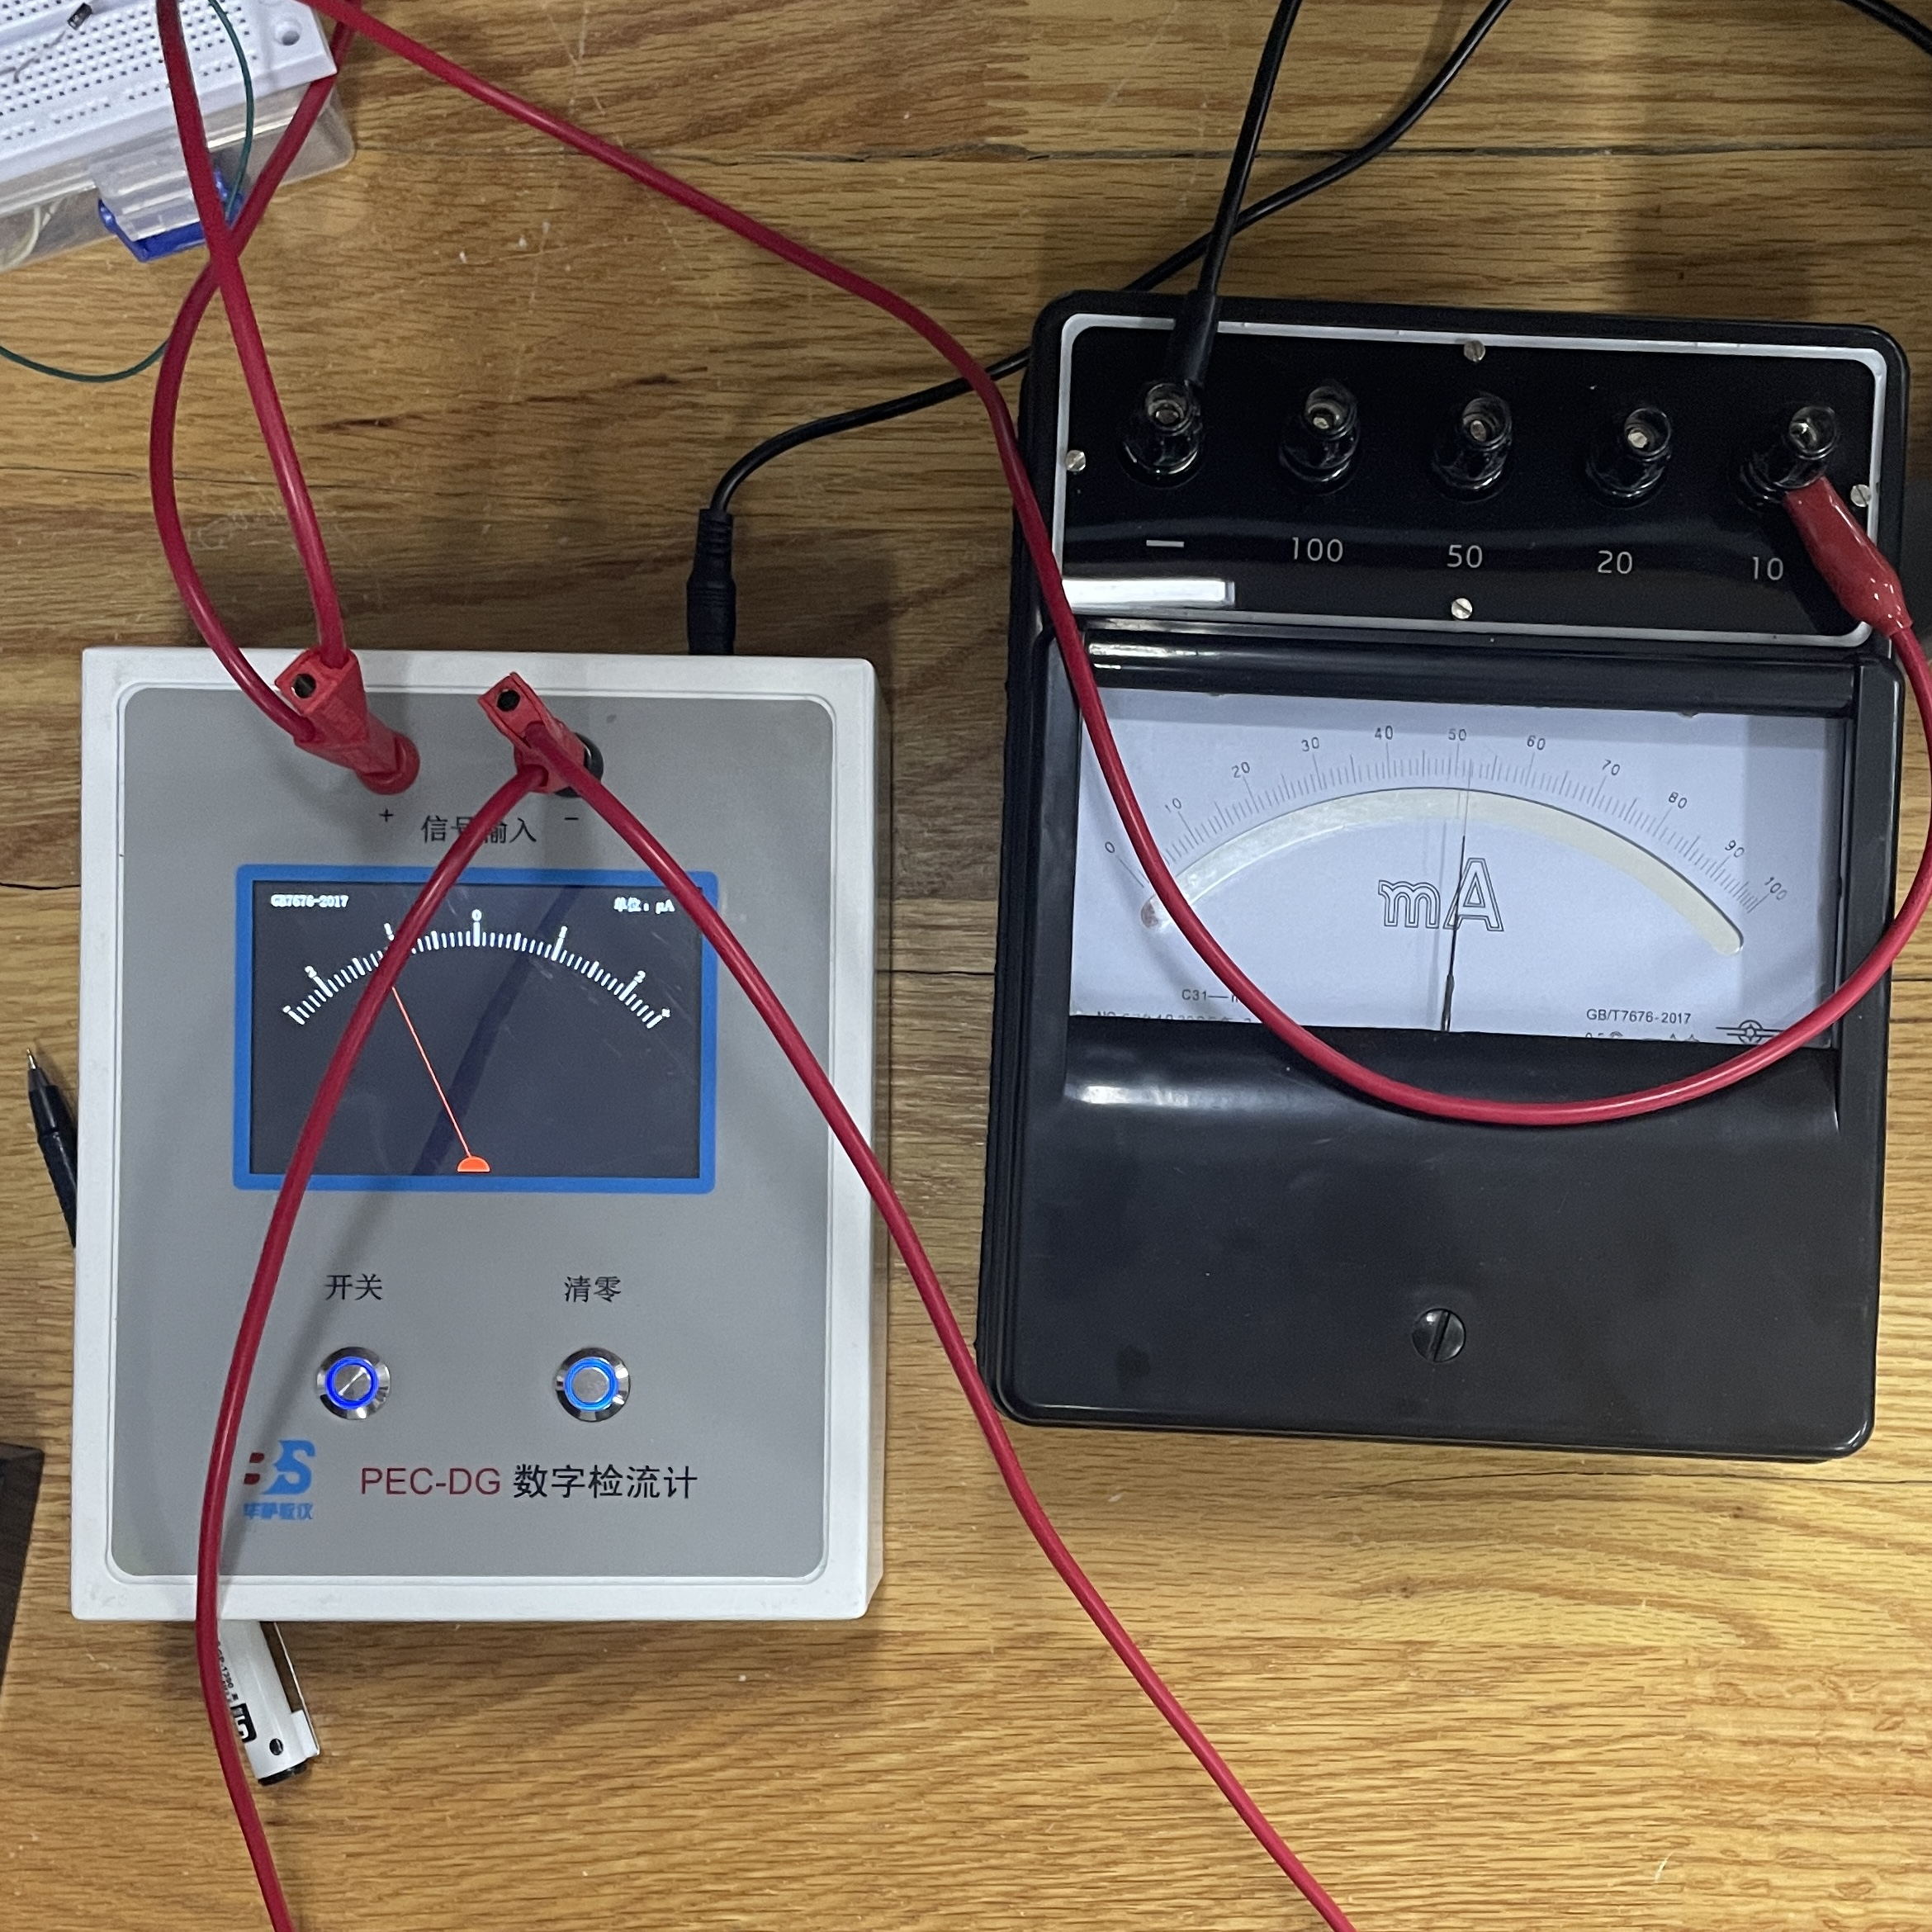
\includegraphics[width=0.95\linewidth]{tp7.jpg}
            \label{tp7.png}
        \end{minipage}
\section{分析与讨论}
    \subsection{定性误差分析}
        \kong \textbf{1.}万用表本身准确性较差，不同量程之间差距较大；\\
        \kong \textbf{2.}万用表分得部分电流，负载等效电阻偏小；\\
        \kong \textbf{3.}二极管等元件不理想，其阻抗对电路有影响。\\
\section{思考题}
    \kong \textbf{1.简述单大电容和小电容$\pi$ 型滤波的优劣。}\\
    \kong \textbf{答：}由整流滤波实验可知，
    单大电容在频率较低，负载阻值较小的情况下适用性较好，负载的直流电压大，功率大，纹波系数小。
    而小电容$\pi$型在频率较高，负载阻值较大的情况下适用性较好，负载纹波系数较小。
    整体上来看，大电容滤波后，输出的直流电压较高，输出功率大，但是纹波系数相较于小电$\pi$型可能偏大；
    小电容$\pi$型滤波效果在频率较高时更好，纹波系数小，但同时直流电压较小。
\end{document}
